\chapter{Sprint Zero}
\minitoc
\newpage
\section*{Introduction}
This chapter will cover the hardware and software environment the project was built on.
\addcontentsline{toc}{section}{Introduction}
\section{Hardware environment}
The project was built on a desktop computer with the following specs :

\begin{itemize}
  \item Processor : Intel i7-7700 Processor (8M Cache, up to 4.20 GHz)
  \item RAM : 8 GB DDR4 3200 MHZ
  \item Graphic card : GTX  1070 8gb GDDR5
  \item Operating system : GTX  1070 8gb GDDR5
\end{itemize}
\section{Software environment}

\hfill \break
\textbf{React \cite{cite3} :} React is a JavaScript library for building user interfaces. React allows developers to create large web applications that can change data, without reloading the page. The main purpose of React is to be fast, scalable, and simple. It works only on user interfaces in the application. This corresponds to the view in the MVC template.


\textbf{Redux \cite{cite4} :} Redux itself is a standalone library that can be used with any UI layer or framework, including React, Angular, Vue, Ember, and vanilla JS. Although Redux and React are commonly used together, they are independent of each other. It's predictable state container for JavaScript apps.

\hfill \break
\hfill \break
\textbf{Node \cite{cite2} :} Node.js is an open-source, cross-platform, JavaScript runtime environment that executes JavaScript code outside a web browser. Node is required to work with react.

\hfill \break
\hfill \break
\textbf{Adobe XD \cite{cite9} :} XD empowers designers with the speed, precision, and quality to seamlessly iterate and share interactive prototypes with team members and reviewers across devices and platforms, including Windows, Mac, iOS, and Android. We will use that to open and work with the wireframes shown previously.

\vfill
\clearpage

\begin{figure}[!ht]
    \centering
    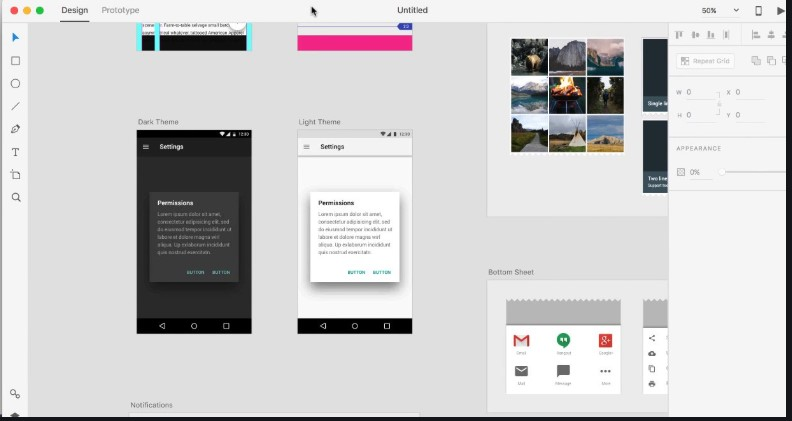
\includegraphics[width=150mm]{adobexd_interface.jpg}
    \caption{Adobe XD interface}
    \label{fig:adobexd_interface}
\end{figure}

\hfill \break
\hfill \break
\textbf{Visual Studio Code \cite{cite7} :} is a code editor developed by Microsoft for Windows, Linux and MacOs. It is one of the best code editors in the market given its speed, the variation of the proposed extensions and the integrated terminal. It also supports several languages and Frameworks such as NodeJS and React.

\begin{figure}[!ht]
    \centering
    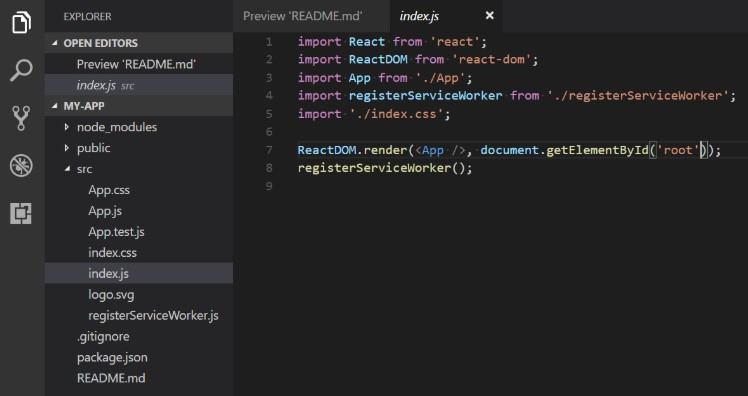
\includegraphics[width=170mm]{visual_code_interface.jpg}
    \caption{Visual Studio interface}
    \label{fig:visual_code_interface}
\end{figure}

\hfill \break
\hfill \break
\textbf{Postman \cite{cite5} :} Postman is a software development tool. It enables people to test calls to APIs. Postman users enter data. The data is sent to a special web server address. Typically, information is returned, which Postman presents to the user.

\begin{figure}[!ht]
    \centering
    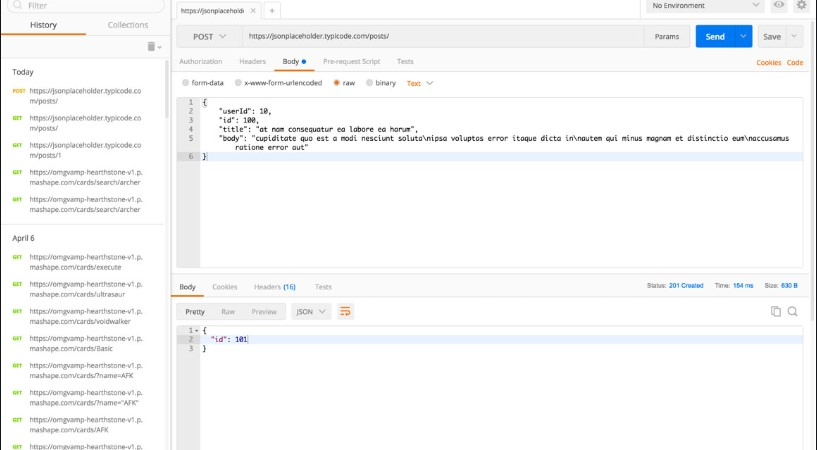
\includegraphics[width=150mm]{postman_interface.jpg}
    \caption{Postman interface}
    \label{fig:postman_interface}
\end{figure}


\hfill \break
\hfill \break
\textbf{Gitlab \cite{cite8} :} is a Git repository hosting service, but it adds many of its own features. While Git is a command line tool, Gitlab provides a Web-based graphical interface. It also provides access control and several collaboration features, such as a wikis and basic task management tools for every project.


\begin{figure}[!ht]
    \centering
    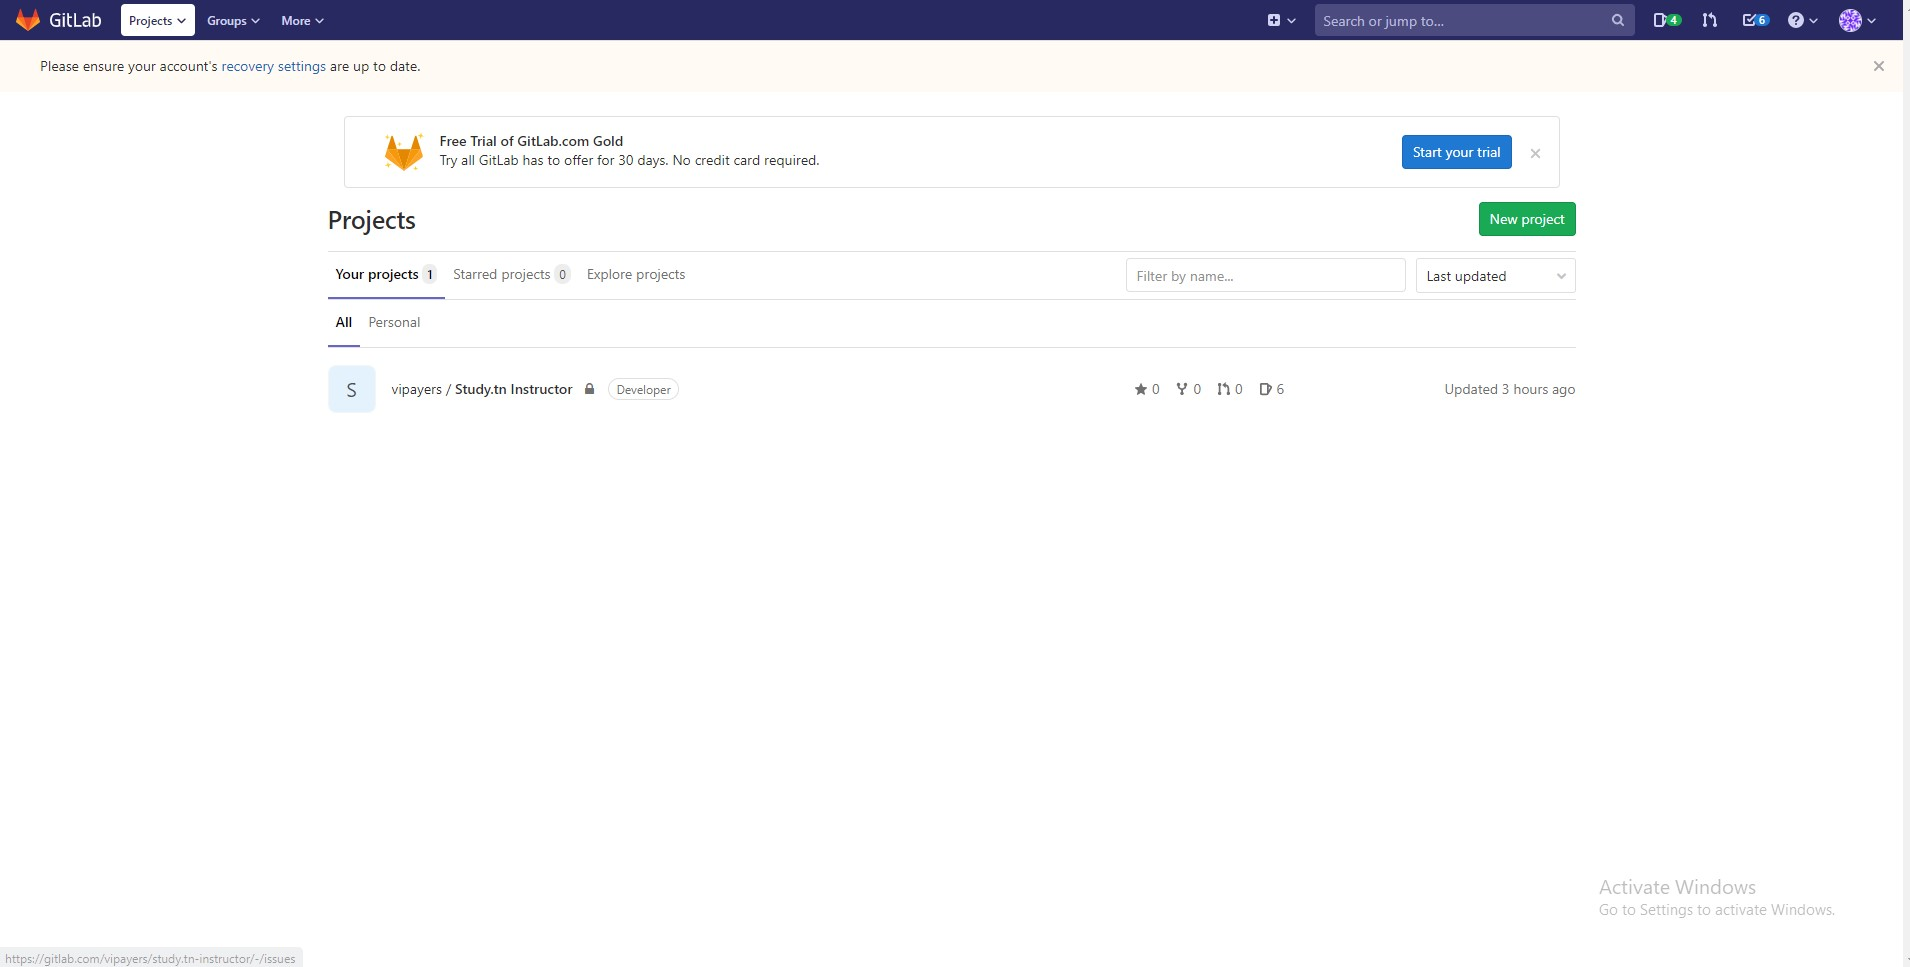
\includegraphics[width=150mm]{gitlab_interface.jpg}
    \caption{Gitlab interface}
    \label{fig:gitlab_interface}
\end{figure}

\vfill
\clearpage

\hfill \break
\hfill \break
\textbf{Slack \cite{cite6} :} Slack is a collaboration hub that can replace email to help you and your team work together seamlessly. It’s designed to support the way people naturally work together, so you can collaborate with people online as efficiently as you do face-to-face.

\begin{figure}[!ht]
    \centering
    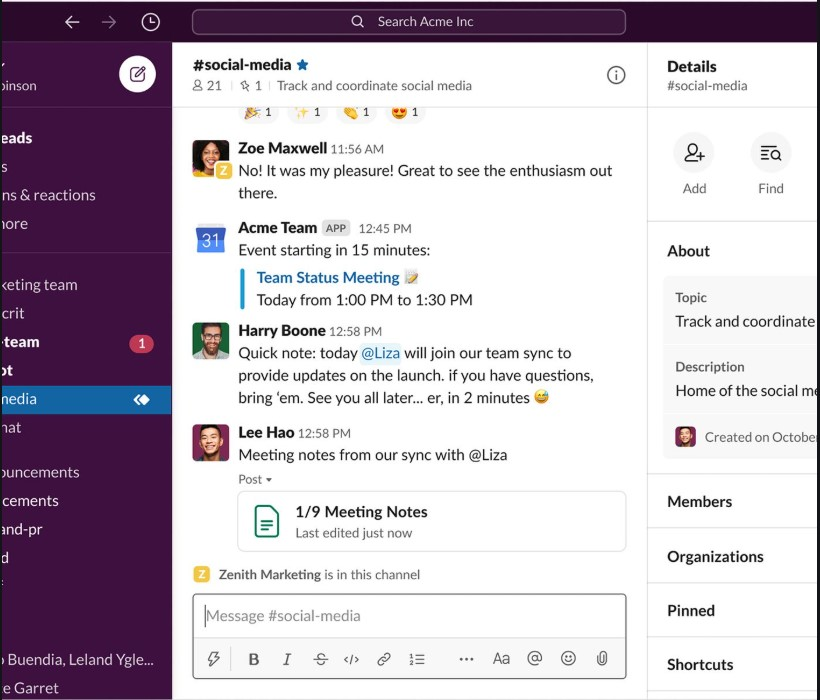
\includegraphics[width=150mm]{slack_interface.jpg}
    \caption{Slack interface}
    \label{fig:slack_interface}
\end{figure}


\section{Application architecture}

\vfill
\clearpage

\begin{figure}[!ht]
    \centering
    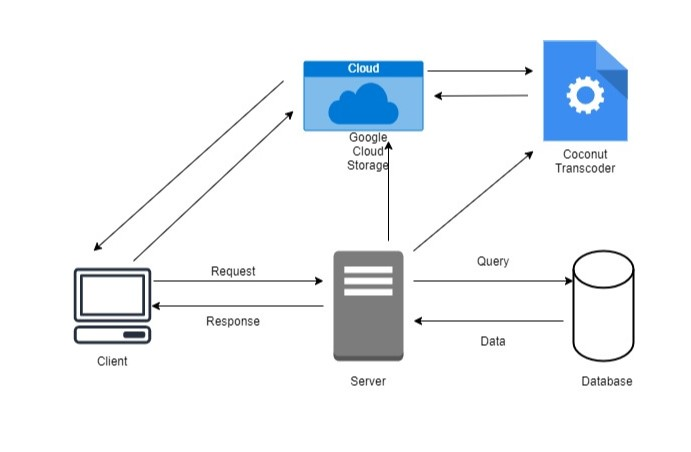
\includegraphics[width=150mm]{project_architecture.jpg}
    \caption{Application architecture}
    \label{fig:slack_interface}
\end{figure}



\section*{Conclusion}
In this chapter, we coved the application architecture, the hardware and software environment used in the project.

\addcontentsline{toc}{section}{Conclusion}